\section{Modélisation numérique}
	\subsection{Motivations et objectifs}
		\subsubsection{Motivations}
			En parallèle de notre étude de la diffusion du véhicule électrique, nous avons travaillé sur le modèle permettant d'évaluer l'impact futur des véhicules électrique sur la consommation globale d’électricité. L'usage de l'outil informatique nous semblant essentiel pour une telle modélisation, étant donné le nombre important de paramètres et la taille de nos échantillons de calculs. Nos efforts se sont donc tournés vers l'élaboration d'un algorithme de calcul capable de produire une courbe représentant la puissance nécessaire à la recharge d'un véhicule électrique au cours du temps.

			En répétant cet algorithme pour un nombre donné de véhicules, et en sommant les puissances calculées, on obtient ainsi une courbe de charge globale pour cette flotte.

			Cette production visuelle nous a semblé la plus à même d'être exploitée dans le cadre de notre étude. Un excés de précision n'aurait pas eu de sens, étant donné la nature statistique de nos données, et les différentes approximations et extrapolations effectuées.

		\subsubsection{Objectifs}
			
			Les objectifs principaux de notre travail de modélisation sont donc :
			
			\begin{enumerate}
				\item Produire un résultat visuel et facilement exploitable de la charge imposée au réseau par une flotte de véhicules électrique, flotte la plus représentative possible de la réalité (Modèle de véhicule, utilisation, ...) 
				\item Permettre de modifier aisément certains paramètres du modèle comme la taille de l'échantillon ou les hypothèses de flexibilité (SmartGrid, Vehicule to grid).
				\item Présenter un algorithme et un cheminement logique clair et détaillé, pour permettre une réutilisation ou une adaptation ultérieure aisée.
			\end{enumerate}

			Nous nous sommes donc rapidement attachés à développer une structure et un organigramme du code assez précis. Ainsi même si des contingences techniques apparaissaient et retardaient notre production d'un programme fonctionnel, et donc de courbes résultats, notre travail pourrait tout de même être une base suffisamment claire et modulaire pour une exploitation future.

	\subsection{Cheminement de pensée}
	
		Après un premier algorithme naïf et peu exploitable, présenté dans le rapport intermédiaire, nous avons choisi d'aborder le problème différemment.
		Pour notre modèle final nous avons décidé de travailler avec une approche plus atomique. Nous avons en effet choisi de considérer les véhicules individuellement, et définis de manière indépendante ---  au lieu d'un véhicule moyen ---  et de faire évoluer chaque véhicule pendant la durée de la simulation selon ses caractéristiques propres.
		
		Cela nous a permis de définir nos véhicules avec une cohérence physique plus grande que lors de l'étude d'un véhicule moyen; par exemple l'utilisation de distributions probabilistes dans l'affectation de certains paramètres permet de simuler le comportement individuel aléatoire d'un véhicule réel.

		Le suivi d'un grand nombre de ces véhicules, permet ensuite d'obtenir une courbe moyenne de consommation pour une flotte.
		
		Cette méthode probabiliste de définition des véhicules s'apparente à une approche de type Monte-Carlo, ou le loi des grands nombres justifie l'utilisation de paramètres aléatoires de loi adaptées pour modéliser des systèmes dont la résolution déterministe est impossible.
		
		Une fois notre approche globale définie nous avons été amenés à préciser les paramètres à étudier et à prendre en compte dans notre modèle. En effet la définition de ces paramètres et leurs dépendances allaient fortement conditionner la manière dont l'algorithme et le code seraient structurés.

		Les paramètres retenus sont donc issus d'un travail en amont, et leur définition a été progressivement affinée au fur et à mesure de l'élaboration du modèle. 

	\subsection{Hypothèses et paramètres}
		
		\paragraph{Hypothèses de base.}
		Tout d'abord, il est important de noter que nous n'avons travaillé que dans le cadre d'une journée de semaine non chômée, avec des véhicules effectuant pour l'essentiel des trajets domicile-lieu de travail. Ce choix de situation, comme nombre des autres hypothèses présentées plus bas, s'est imposé a nous pour des questions de simplicité de modélisation. De plus il nous a semblé le plus représentatif d'une situation réelle.
		
		Afin de représenter les déplacements du véhicule, nous avons retenu trois lieux de stationnement où l'utilisateur est susceptible d'utiliser une borne de recharge :
		\begin{itemize}
			\item Sa maison ;
			\item Son lieu de travail;
			\item La voie publique, qui regroupe toutes les autres destinations possibles (centre commercial, centre ville, école des enfants, lieu de loisir, etc.).
		\end{itemize}
		
		Nous avons aussi considéré quatre états de mouvements possible pour un véhicule : 
		\begin{itemize}
			\item En train de rouler : le véhicule se déplace;
			\item Garé non branché  : le véhicule est à l'arrêt et n'est pas relié à une borne de recharge;
			\item Branché en charge  : le véhicule est à l'arrêt, relié à une borne, et se recharge;
			\item Branché par en charge : le véhicule est à l'arrêt, relié à une borne, mais ne se recharge pas (par utilisation d'une recharge différée, ou parce que le véhicule est pleinement chargé).
		\end{itemize}
		
		
		\paragraph{Paramètres physiques.} Nous avons retenu cette liste de paramètres physiques caractérisants nos véhicules :
		
		\begin{itemize}
			\item Le type de véhicule, à savoir : Véhicule particulier (VEP), Véhicule d'entreprise (VEE), ou Véhicule d'auto partage (VAP);
			\item Le modèle de véhicule : nous en avons retenus 5 différents (Renault Zoé, Nissan Leaf, Bolloré Blue Car, Smart ForTwo et Tesla Model S);
			\item La capacité de la batterie du véhicule (en \si{\kilo\watt\hour}) et la consommation (en \si{\kilo\watt\hour\per\kilo\meter}), dépendant directement du modèle de véhicule;
			\item La vitesse : supposée constante pour chaque véhicule, elle est initialisée pour chaque véhicule à partir d'une distribution gaussienne centrée à \SI{38,75}{\kilo\meter\per\hour}, valeur moyenne pour les déplacements des véhicules en France, et un écart type de 10.
			\item La longueur d'un trajet : de même que pour la vitesse, nous effectuons l'hypothèse que pour un véhicule donné, tous ses trajets font la même longueur. Cette longueur est tirée selon la répartition statistique des distances parcourues par les véhicule en France;
			\item Le nombre de trajets effectués en une journée : de même que pour les deux paramètres précédents, chaque véhicule effectue un nombre de trajet fixe, initialisé selon une distribution gaussienne, dont les paramètres sont issus des données statistiques à notre disposition;
			\item L'accès aux bornes : chaque véhicule a éventuellement à sa disposition une borne au différentes positions possibles (ex : le VEP \no{}1 possède une borne chez lui, mais ni au travail, ni dans les lieux public qu'il fréquente, tandis que le VEP \no{}2 possède une borne chez lui, et également sur son lieu de travail ou son employeur a mis en place des bornes a disposition des employés). Cette répartition est issue de données statistiques à priori, mais peut être modulée pour générer des projections dans divers cas futurs.  
			\item L'état de charge (State of Charge ou SOC) : évoluant au cours du temps, évalué en pourcentage de la capacité totale de batterie;
			\item L'état de mouvement du véhicule et sa position, tels que définis ci-dessus;
			\item Les horaires de trajets du véhicule : à partir de données statistiques sur les horaires de trajets réels, et du nombre de trajets qu'il va effectuer, chaque véhicule se voit affecter une liste d'horaires à laquelle il est censé partir de sa position actuelle (s'il est insuffisamment chargé il attendra le temps nécessaire à sa recharge).
			\item La puissance de recharge d'un véhicule: actuellement tous les véhicules ont le même profil de charge, avec une puissance nominale délivrée par le réseau constante fixée à \SI{3,5}{\kilo\watt}.
		\end{itemize}
		
		Dans cette liste de paramètres apparaissent déjà un certain nombre d'hypothèses, qui peuvent sembler assez fortes, sur la définition d'un véhicule : vitesse et longueur des trajets fixes ou encore horaires des trajets définis à l'avance et pour toute la durée de la simulation.
		
		Ces hypothèses nous ont semblé nécessaires pour pouvoir créer un algorithme d'une complexité raisonnable. De plus ces écarts à la réalité physique d'un véhicule sont compensés par l'utilisation d'un grand nombre de véhicules de paramètres aléatoires lors des modélisations. Comme les variables aléatoires sont choisies en adéquation avec les données statistiques réelles, la loi des grands nombre assure la convergence de nos simulations avec des véhicules virtuels vers les valeurs attendues dans la réalité.
		
		\paragraph{Hypothèses supplémentaires.} A ce qui a été présenté précédemment nous avons ajoutés un certain nombre de variables et d'hypothèses qui ont un sens physique, mais dont les définitions relèvent plus de l'arbitraire et du \emph{qualified guess} que de données statistiques. Tous ces paramètres font partie de la définition d'un véhicule et même si certains évoluent au cours de la simulation l
		
		\begin{itemize}
			\item Les destinations des véhicules sont choisies a priori. 
				\begin{itemize}
				
					\item Pour un VEP nous avons considéré divers cas horaires :
					\begin{itemize}
						\item de 7h à 11h tous les trajets d'un particulier le conduise sur son lieu de travail, et dans le cas ou il est déjà sur son lieu de travail un trajet l’amène dans un lieu public (déplacement professionnel);
						\item de 11h à 14h un trajet depuis un lieu public (ou il a pris son repas par exemple) l'amène sur son lieu de travail, et un trajet depuis sa maison ou son lieu de travail l'amène aléatoirement à l'un des deux autres lieu possibles (trajet travail->maison pour le repas par exemple, ou maison->lieu extérieur pour aller chercher les enfants à l'école);
						\item de 0h à 7h et de 14h à 24h un trajet depuis la maison l'amène sur un lieu public (école des enfants, sortie le soir, courses, etc.), et tout autre trajet a pour direction la maison.
					\end{itemize}
					
					\item Pour un VEE il y a aussi une distinction horaire, mais plus simple :
					\begin{itemize}
						\item s'il est plus de 18h le véhicule rentre sur son lieu de travail, qui dans le cas d'un véhicule d'entreprise est sa base de départ;
						\item sinon tous les déplacements sont des déplacements professionnels qui vont vers un lieu public.
					\end{itemize}
					
					\item Enfin pour un véhicule d'auto-partage le trajet est aléatoirement vers un lieu public, ou un lieu de travail.
				\end{itemize}
			Ces destinations sont déterminées lors de l'initialisation d'un véhicule, et un parcours de ce tableau vérifie que chaque véhicule accède à une borne au cours de ses trajets, quitte à recommencer la création du véhicule si celui-ci ne trouve pas de bornes sur son trajet.
			\item Nous avons imposés certaines contraintes sur la répartition des bornes des VEE et VAP :
				\begin{enumerate}
					\item Un VEE aura toujours une borne sur son lieu de travail;
					\item Un VAP aura toujours une borne disponible dans un lieu public (nous faisons l'assomption que l'utilisateur le ramène toujours près d'une borne après utilisation).
				\end{enumerate}
			\item Pour prévenir la "panne sèche" d'un véhicule au cours d'un trajet, nous avons introduit une variable \texttt{socMin} qui contient l'état de charge minimum requis pour voyager jusqu’à la prochaine borne. Le calcul de cette variable est simplifié par la connaissance au préalable des destinations, de l'accès au bornes et de la distance des trajets. Cela peut paraitre un peu artificiel dans le cadre de notre modèle, mais dans la réalité un utilisateur a la plupart du temps connaissance de ses capacités de recharge au cours du trajet, et les prends en compte lorsqu'il débranche ou non son véhicule. Nous supposons que le véhicule ne peut redémarrer s'il n'a pas atteint un état de charge supérieur ou égal a \texttt{socMin}. 
		
			
		\end{itemize}

	\subsection{Description de l'algorithme}
		
		L'algorithme se décompose donc en deux parties distinctes :
		\begin{enumerate}
		
			\item Tout d'abord l'initialisation du véhicule, qui doit définir tous les paramètres décrits ci-dessus, et s'assurer que ceux ci caractérisent un véhicule fonctionnel, c'est à dire un véhicule qui a accès à des bornes, qui peut faire tous ses trajets, etc. Cette partie est organisée de manière très linéaire, avec une succession d'affectation et de vérifications qui aboutissent à la définition du véhicule. Elle est effectuée une fois par véhicule. Sa structure est détaillée au paragraphe \ref{sec.descrInit}
			
			\item Ensuite la partie d'évolution. Elle consiste essentiellement en une série de tests sur l'état du véhicule (quel est son état de mouvement, son état de charge, le nombre de trajets à effectuer, etc) qui modifient ces mêmes paramètres d'état selon les résultats obtenus. C'est une boucle que chaque véhicule parcours une fois par pas de temps. C'est dans cette partie que va être modifié le tableau résultat \texttt{puissanceReseau}, qui contient la puissance nécessaire à la recharge de la flotte considérée pour chaque pas de temps. La structure de cette boucle est illustrée par les diagrammes \ref{fig.flowPrincipal} et \ref{fig.flowTransition}, et commentée dans le paragraphe \ref{sec.descrSimulation}.
		
		\end{enumerate}
		
		\subsubsection{Initialisation des véhicules \label{sec.descrInit}}
			
			Comme mentionné ci-dessus, l'initialisation des véhicule est un processus séquentiel, où l'ordre des étapes dépend de manière fondamentale des dépendances entre les paramètres. Une partie importante de sa conception a donc été de bien distinguer ces dépendances pour pouvoir écrire un programme ayant du sens physiquement, et avec des étapes les plus élémentaires possibles.
			
			Voici donc les étapes de l'initialisation d'un véhicule :
			
			\begin{enumerate}
				\item Initialisation du SOC (\texttt{soc}) à 100 $\percent$ : ab initio tous les véhicules sont chargés.
				\item L'état de mouvement (\texttt{etatMouvActuel}) est défini comme branché en charge (\texttt{BRANCHE\_EN\_CHARGE}).
				\item L'état de mouvement suivant, variable interne utilisée dans la boucle d'évolution, est défini de même : \texttt{etatMouvSuivant = BRANCHE\_EN\_CHARGE}.
				\item Initialisation de la distance parcourue et du nombre de trajets effectués par le véhicule à 0 : \texttt{distanceParcourue = 0; nbTrajetsEffectues = 0}.
				\item Initialisation du type de véhicule (\texttt{typeVehicule}) : VEE, VAP ou VEP.
				\item Initialisation de la position (\texttt{position}) de départ du véhicule.
				\item Définition du modèle du véhicule (\texttt{modele}).
				\item Initialisation de la capacité et de la consommation du véhicule, qui dépendent du modèle de véhicule (\texttt{consommation}, \texttt{capacite}).
				\item Initialisation de la vitesse de déplacement et de la longueur des trajets tels que présentés plus hauts (\texttt{vitesse},\texttt{longueurTrajet}).
				\item Initialisation du nombre de trajet par jour (\texttt{nbTrajets}).
				\item Disponibilité des bornes : maison OUI/NON, lieu de travail OUI/NON, lieu public OUI/NON. (tableau \texttt{accesBornes}).
				\item Test de la disponibilité d'au moins une borne pour le véhicule.
				\item Calcul des horaires de départs (\texttt{horaireDepart})
				\item Vérification qu'il n'y a pas chevauchement entre un trajet et le suivant, c'est à dire que le véhicule à bien fini le trajet précédent au moment ou il doit effectuer le suivant.
				\item Vérification que le véhicule passe bien par une borne au cours de la journée.
				\item Initialisation du SOC minimal (\texttt{socMin}) à la valeur nécessaire pour atteindre la prochaine borne.
			\end{enumerate}	
	
			Cette initialisation correspond au constructeur \texttt{Vehicule::Vehicule(int deltaT)} de la classe \texttt{Vehicule.cpp}. Le paramètre \texttt{deltaT} correspond au pas de temps de la simulation. Une fois le véhicule correctement initialisé nous le faisons évoluer dans la boucle de simulation.
	
		\subsubsection{Boucle de simulation \label{sec.descrSimulation}}
			
			\paragraph{}L'organisation logique de la partie évolutive de la simulation est présentée dans le diagramme ci dessous (figure \ref{fig.flowPrincipal}). Pour plus de lisibilité le bloc transition est présenté à part, dans la figure \ref{fig.flowTransition}. Ces deux blocs correspondent respectivement aux méthodes \texttt{double Vehicule::simulation(int temps, int deltaT)} et \texttt{int Vehicule::transition(int temps, int deltaT)} de la classe \texttt{Vehicule.cpp}. L'opération de bouclage de la méthode \texttt{simulation} est effectué lors de son appel dans la fonction \texttt{main}.
			
			La méthode \texttt{simulation} prend en paramètre le \texttt{temps} actuel --- mesuré en nombre de pas de temps \texttt{deltaT} --- et retourne la puissance demandée par le véhicule sur lequel on appelle cette méthode a l'instant \texttt{temps}.
			La méthode \texttt{transition} prend les mêmes paramètres que \texttt{simulation} et retourne un entier correspondant à l'état de mouvement dans lequel sera le véhicule au prochain pas de temps (\texttt{etatMouvSuivant}).
			
			\begin{figure}[h]
				\centering
				\caption{Logigramme de la méthode \texttt{simulation} \label{fig.flowPrincipal}}
				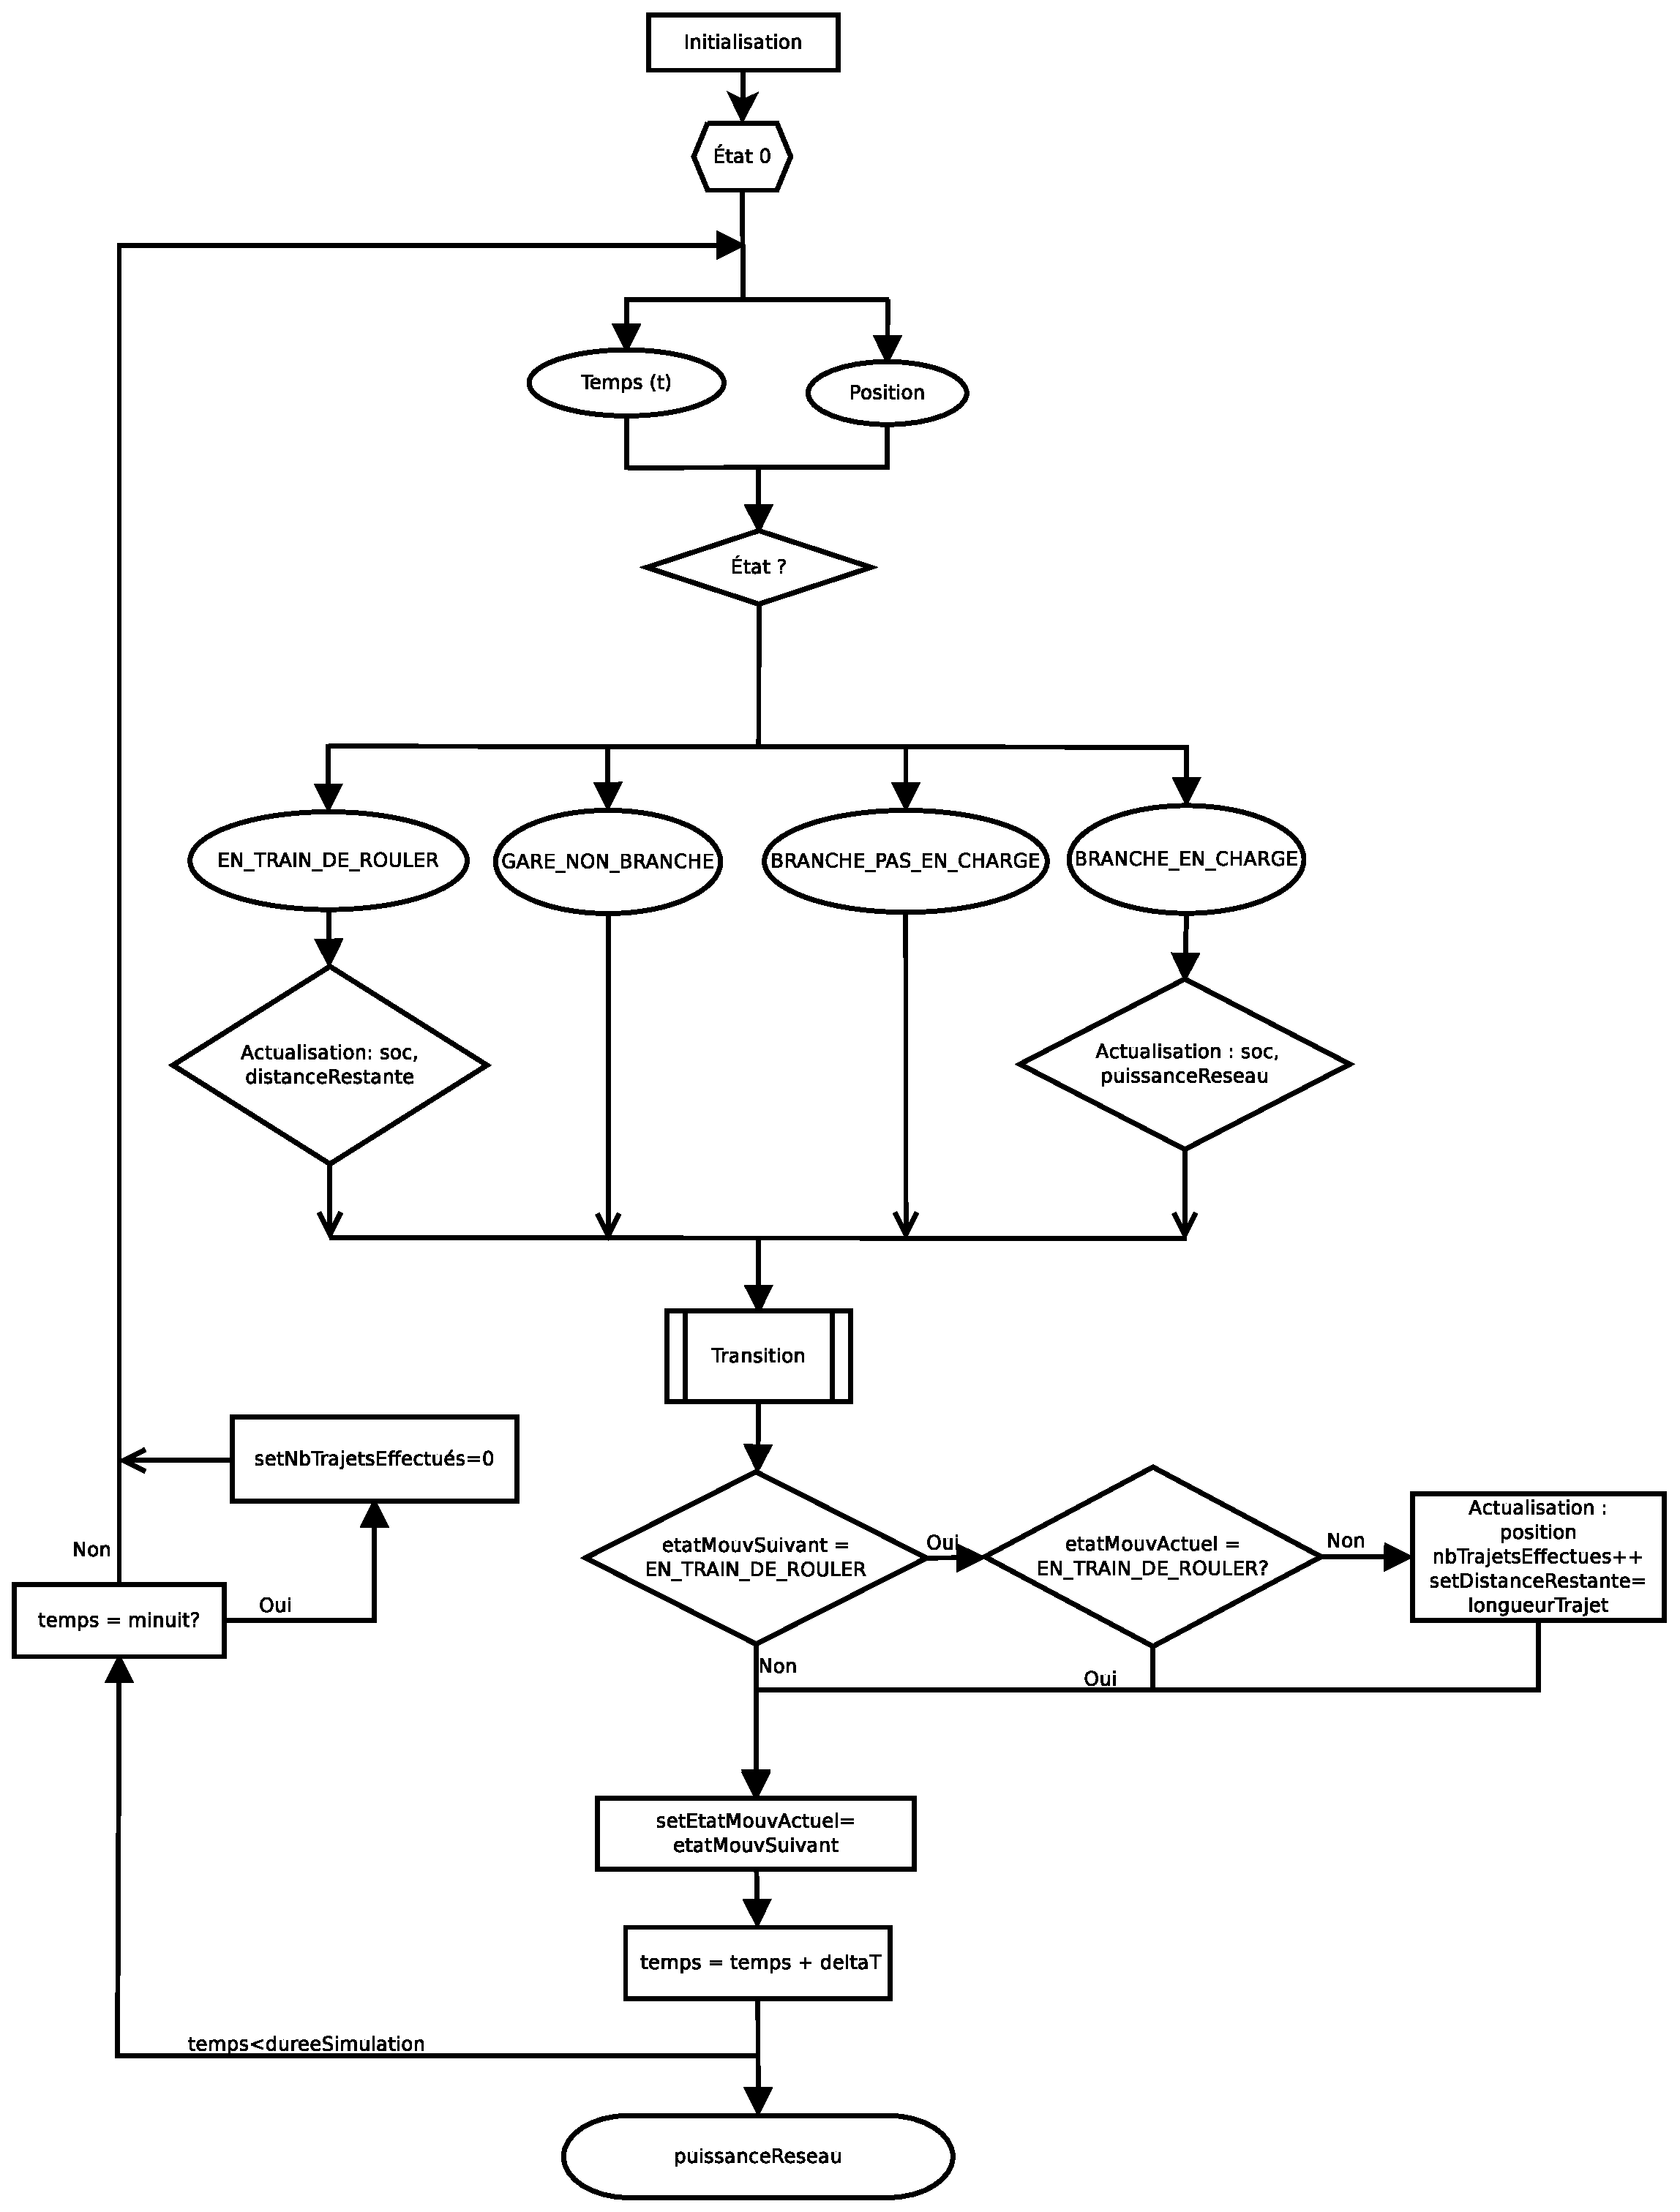
\includegraphics[height=0.9\textheight]{fig/flowPrincipal.eps}
			\end{figure}
			\begin{figure}[h]
				\centering
				\caption{Bloc Transition \label{fig.flowTransition}}
				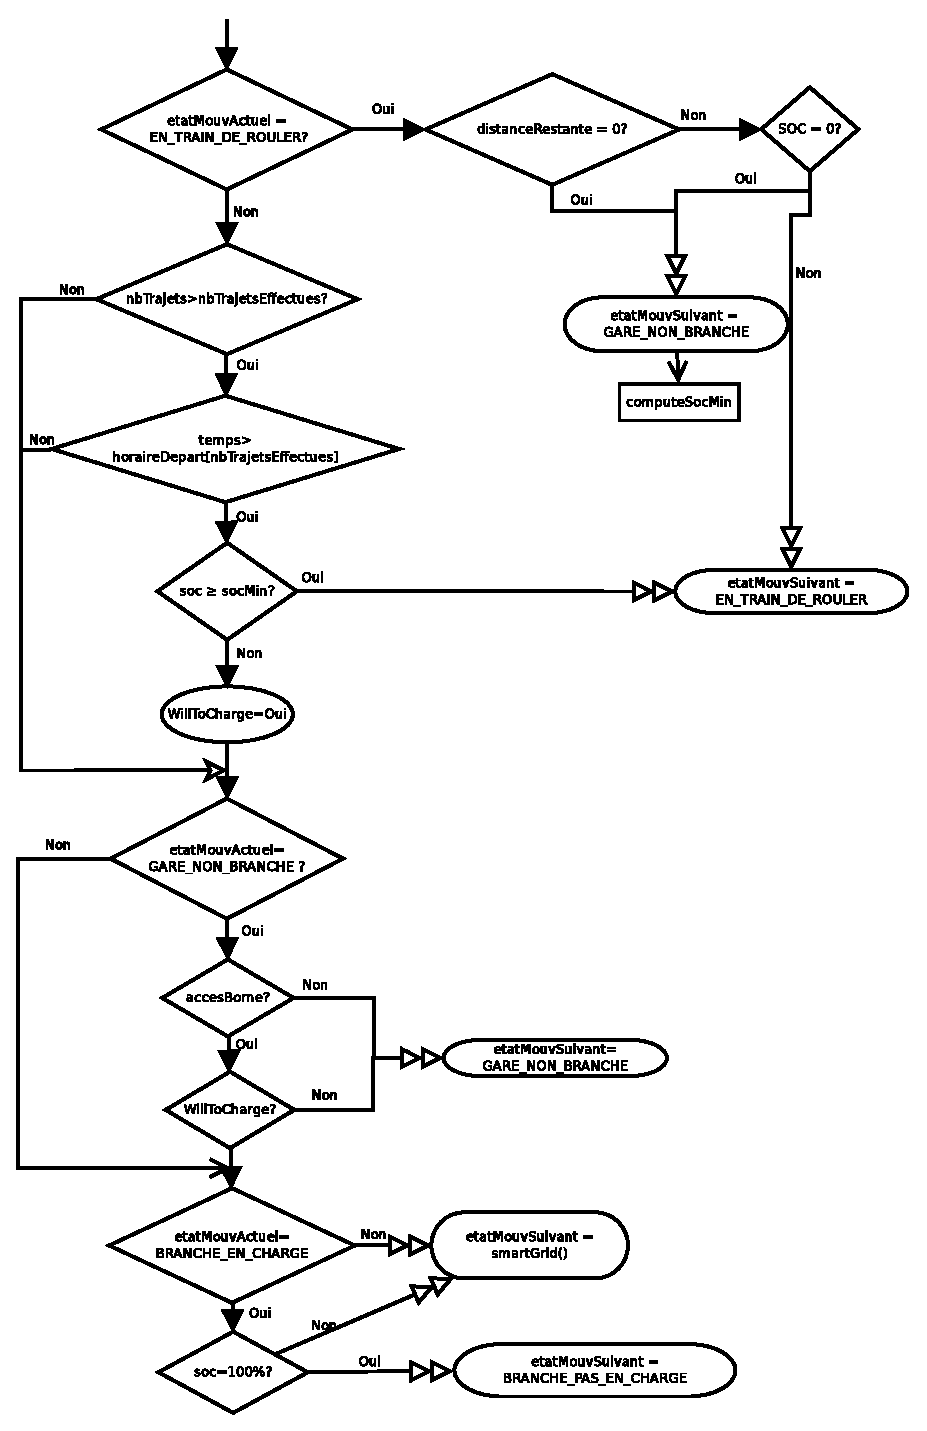
\includegraphics[height=0.9\textheight]{fig/flowTransition.eps}
			\end{figure}
			
			
			Dans l’organigramme de la méthode \texttt{transition} on observe deux variables qui n'ont pas encore été décrites.
			
			\paragraph{}La première,  \texttt{willToCharge}, est un booléen qui décrit de manière sommaire le comportement de l'utilisateur. On fait l'hypothèse d'un utilisateur rationnel qui ne met son véhicule en charge que lorsque l'autonomie de celui-ci ne lui permet pas de faire les trajets à venir. On simule ainsi le comportement réel des utilisateurs qui, d'après nos données, ne chargent pas leur véhicule de manière systématique, mais en moyenne tous les trois jours.
			
			\paragraph{}La deuxième est la fonction \texttt{int smartGrid(Vehicule* v)}. Cette fonction est là pour prendre en compte tous les aspects de \emph{Smart Grid}, \emph{Vehicle to grid}, effacement de charge, etc. C'est dans cette fonction que seront implémentés les différents cas possibles (\emph{use cases}) de monitoring de la charge d'un véhicule. Les \emph{use cases} que nous avons utilisés, et leur implémentation, sont décrits dans la paragraphe \ref{sec.useCases}. 
			
			D'un point de vue pratique, cette fonction prend pour argument le véhicule qui est actuellement dans la boucle et retourne un entier qui correspond à un état de charge (\texttt{BRANCHE_EN_CHARGE} ou \texttt{BRANCHE_PAS_EN_CHARGE}) selon l'état du véhicule et la méthode d'effacement utilisée. Cette méthode sera le plus souvent imposée par le fournisseur d’électricité dans la réalité.
			
			\paragraph{} Lors de l'appel de la fonction \texttt{main}, la fonction principale du programme, celle ci prend différents arguments :
			\begin{itemize}
			\item La longueur du pas de temps, \texttt{deltaT}, en minutes;
			\item Le nombre $D$ de pas de temps que va durer la simulation;
			\item Le nombre $N$ de véhicules a générer pour la simulation.
			\end{itemize}
			
			Le tableau \texttt{puissanceReseau}, de taille $D$  et indexé par les pas de temps de la simulation, est ensuite initialisé. Chaque case contiendra la puissance requise par l'ensemble de la flotte modélisée pour se recharger à l'instant correspondant.
			
			Ensuite la fonction est basiquement une double boucle :
			\begin{enumerate}
			\item Une première boucle sur la taille de l'échantillon, qui génère un véhicule par étape et le fait passer dans la deuxième boucle;
			\item La deuxième boucle est celle décrite dans l'organigramme \ref{fig.flowPrincipal}, indexée par les pas de temps successifs, ou a chaque itération la fonction \texttt{simulation} rempli la case correspondante de \texttt{puissanceReseau}.
			\end{enumerate}
			
			En sortie, on obtient donc un tableau contenant toutes les informations nécessaires au tracé de la courbe de charge imposée par cette flotte au cours du temps.
			%	\begin{tikzpicture}
% style des noeuds
\tikzstyle{etat} = [diamond, draw]
\tikzstyle{test} = [rectangle, draw]
\tikzstyle{instruct} = [rectangle, draw, rounded corners=4pt]
% style des flèches
\tikzstyle{suite} = [->, >=stealth', thick, rounded corners=4pt]

% placement des noeuds
\node[instruct] (initialisation) at (0,0) {Initialisation}
\node[etat] (etat0) at (0,-1) {\'Etat $t$}
\node[test] (whichState) at (0,-2) {etatMouvement ?}

% placement des flèches
\draw[suite] (initialisation) -- (etat0)
\draw[suite] (etat0) -- (whichState)
\end{tikzpicture}
		
		
		\clearpage
	\subsection{Résultat}

2 jours == 10 jours mentionner